\label{sec:part_1_method}

We shall adopt the pipeline introduced in the original paper to reproduce their results.
In the upcoming subsections, we shall describe the methodologies and highlight the issues and/or limitations in their work.
The results in this section are extracted from \texttt{reproduction.ipynb}.

\subsubsection{Feature extraction}

Prior to this stage, the \textbf{Data Preprocessing} stage flattens 12–lead ECG diagrams into a single vector, i.e. $(1000 \times 12) \rightarrow (12000,)$.
We also noticed a critical typo issue in the original paper, stating that ``ECG signal has 21000 dimensions'', but in fact, it only has 12000 dimensions, as written just before their section C in ``III. METHODS''.
A visualisation of the first flattend ECG record in the dataset is, note that difference with the \textbf{Fig. \ref{fig:12_lead_ecg}}.

After that, we apply the \texttt{neurokit2} package \cite{Makowski2021neurokit} to extract the features, i.e. $(12000,) \rightarrow (16, N)$, where $N$ is the number of peaks detected, and vary among ECG records.
Moreover, as highlighted in \cite{GOLDBERGER2018xi}, each lead in the 12-lead ECG are all comprising of the same peak amplitudes, intervals and segments as shown in \textbf{Fig. \ref{fig:ecg-waveform}}, though each of which offers different viewpoints.
However, as described, they flatten the 12 leads prior to extracting features, and thus, do not exactly conform to the medical meaning of these features. Therefore, it results in two hurdles they acknowledged later.

Besides, they do not present mathematical expressions to compute the intervals, hence, we shall rely on their description to work out these features, as below.
PQ = Q - P, ST = T - S, QT = T - Q, PR = R - P, QRS = S - Q and $\text{RR} = R_i - R_{i - 1}$, where $R, P, Q, S, T$ are five peak amplitudes.

The 16 features extracted by the following process. Firstly, we detect the R peak locations by using \texttt{ecg\_peaks()}, subsequently utilise \texttt{ecg\_delineate()} to obtain other peak locations using the R peaks as reference, and we set \texttt{method = "peak"} as \cite{sinha2023dasmcc} does not clearly specify,
eventually calculate the intervals/segments by applying the expressions shown above. There exist null values during this process, and thus, we always take this issue into account at every step.

\begin{table}[H]
    \centering
    \caption{16 features extracted by \texttt{neurokit2} \cite{sinha2023dasmcc}.}
    \label{tab:extracted_features}
    \begin{tabular}{lr}
        \toprule
        Feature group & Feature's name \\
        \midrule
        Peak's positions & P\_loc, Q\_loc, R\_loc, S\_loc, T\_loc     \\
        Peak's amplitude & P\_amp, Q\_amp, R\_amp, S\_amp, T\_amp     \\
        Intervals and segments & PQ, ST, QT, PR, RR, QRS     \\
        \bottomrule
    \end{tabular}
\end{table}

\subsubsection{Data preparation}

As reported in the original paper, the difficulties do exist.
First, there are 280 records (roughly 1.7\%) whose 16 features contain missing values.
Second, the number of R peaks across features differ significantly, i.e. 67 distinct feature lengths (min 0, median 12, max 81).
Third, in 157 ECG records, the 16 features do not share the same number of R peaks. For brevity, we shall refer to R peaks as beats.

\begin{figure}[H]
    \centering
    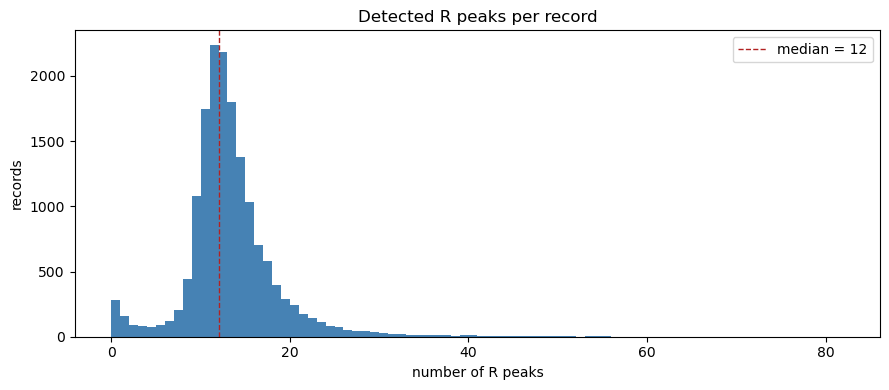
\includegraphics[width=1\textwidth]{figures/part1/peaks_per_record.png}
    \caption{Number of R peaks across 16244 ECG records.}
    \label{fig:peak_per_record}
\end{figure}

We shall resolve the above–mentioned issues as follow, strictly obey the order. First, we apply the Forward Filling (\texttt{ffill}) technique to impute the missing values presented in the dataset.
Then, we equate the feature lengths across the dataset; however, \cite{sinha2023dasmcc} is unclear about this, we shall apply the median length, i.e. 12, which we believe it may balance between unnecessarily padding to compensate the length and dropping useful signals presented.
Next, we flatten the features, i.e. $(16 \times 12) \rightarrow (192,)$.

We further realise that, an early application of \texttt{np.diff(R, prepend = np.nan)}, to compute RR, introduces some null values that \texttt{ffill} may again impute null values to the succeeding elements.
Therefore, we complement the pipeline with another \texttt{ffill()}. Moreover, there exists a column with null values everywhere, and thus, we drop this column. Eventually, the number of features passed to the upcoming stages is $191$.
These subtle issues are not clearly explained in \cite{sinha2023dasmcc}. Then, we encode the diagnostic classes with numbers, in lieu of applying \texttt{LabelEncoder()} we strictly adhere to the following rules, established in \cite{sinha2023dasmcc}.

\begin{table}[H]
    \centering
    \caption{Label encoding of diagnostic classes \cite{sinha2023dasmcc}.}
    \label{tab:label_encoder}
    \begin{tabular}{lr}
        \toprule
        Class & Numerical label \\
        \midrule
        NORM & 0 \\
        MI & 1 \\
        STTC & 2 \\
        HYP & 3 \\
        CD & 4 \\
        \bottomrule
    \end{tabular}
\end{table}

Next, we leverage the \texttt{train\_test\_split()} from \texttt{sklearn} to randomly partition the dataset into train/test sets using the 8/2 ratio.
Nonetheless, the paper is unclear about what \texttt{random\_state} they used and whether the attempted to partially resolve the imbalance issue by setting \texttt{stratify} during the split.
We shall use \texttt{random\_state = 42} and do not apply \texttt{stratify} to get the most imbalanced train/test sets, at least more imbalanced than applying \texttt{stratify}.
Therefore, the imbalancing issue is somewhat preserved in both partitioned train and test sets, as demonstrated below.

\begin{figure}[H]
    \centering
    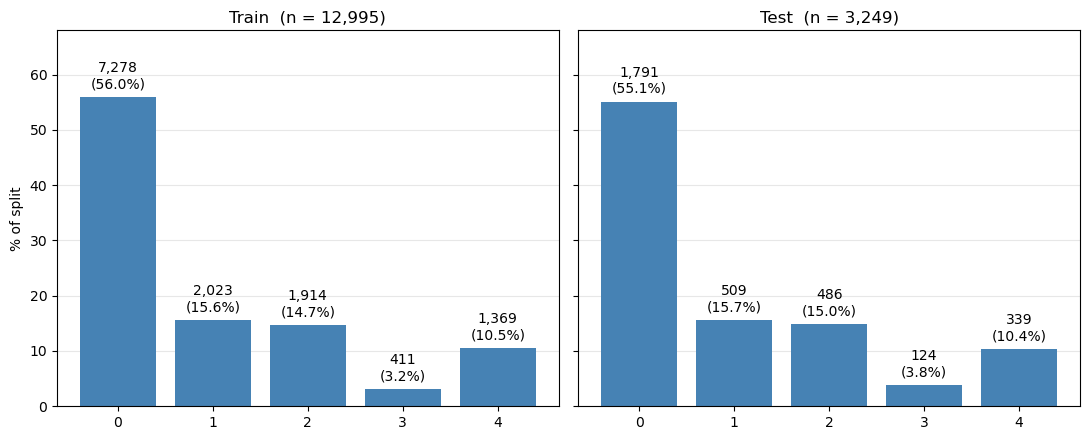
\includegraphics[width=1\textwidth]{figures/part1/train_test_class_distribution.png}
    \caption{Class distribution of train and test sets}
    \label{fig:train_test_class_distribution}
\end{figure}

\subsubsection{Data augmentation}

It has been recognised and extensively studied in ML community that, performance of ML algorithms are adversely influenced by the presence of underrepresented data and/or skewness of class distributions \cite{learning-imbalanced}.
Consequently, this class–imbalanced dataset amplifies the models' biases towards predominant classes and may misclassify classes with fewer samples \cite{sinha2023dasmcc}.

Having splitted the dataset, the original paper resolves class–imbalance issue by the utilisation of SMOTE, which stands for Synthetic Minority Over–sampling Technique \cite{SMOTE}.
A more thorough description of SMOTE can be found in \cite{SMOTE}. In brief, given our dataset $\mathcal D \triangleq (\mathcal X, \mathcal Y)$, consider the feature space $\mathcal X$, it randomly picks a sample, $\mathbf x_i \in \mathcal X$, from the minority class, $\mathbf y_i \in \mathcal Y$, then again, randomly selects one of its $k$ nearest neighbours by \texttt{KNN}, says $\mathbf x_j \in \mathcal X$, and of couse, $\mathbf y_j = \mathbf y_i$.
Next, it computes their difference, $\mathbf d = \mathbf x_i - \mathbf x_j$, and complementing the current dataset $\mathcal D$ by $\mathcal X \leftarrow \mathcal X \cup \left\{ \mathbf x_i + \alpha \mathbf d \right\}$ and $\mathcal Y \leftarrow \mathcal Y \cup \left\{ \mathbf y_i \right\}$, where $\alpha \sim U(0, 1)$.
Repeating this process untill all classes in $\mathcal Y$ share the same number of samples. We utilise \texttt{imblearn} as an alternative to manually re-implementing this technique.
Also, we use the \texttt{random\_state = 42}, since the original paper does not mention therein.
Additionally, they also mention the feature scaling at the end of section ``III.E'', though absence of the method, and thus, we shall apply \texttt{StandardScaler()} prior to \texttt{SMOTE}.

We further note that, the class–imbalance handling strategy is only applied to the train set, while the test set is left unchanged, otherwise, we would falsely report the actual performance of our models on the test set.
Later on, we shall show that, following this approach cannot reproduce their results, whereas violating this approach, i.e. \texttt{SMOTE} before train/test split yields closer reproduced results.

Another unclear statement in their paper, they mentioned the process is applied to ``80\% of training data, which are selected randomly in each fold of the 10–fold cross–validation''.
This is ambiguous, since in a standard 10–fold CV splits into 90\% train and 10\% test.



\subsubsection{Modeling}

We also noted another critical issue of the original paper, in their abstract, they stated the use of \texttt{AdaBoost}, also another typological error here, but later in the main body, they use \texttt{CatBoost}.
Due to this inconsistency, we shall evaluate both \texttt{CatBoost} and \texttt{AdaBoost}. Up to our knowledge, \texttt{CatBoost} was originally made to improve accuracy for datasets composing of predominant number of categorical features \cite{CatBoost} (though it can still work in the presence of numerical features), while our feature space is continuous, rather than discrete.

In this experiment, we use, from \texttt{sklearn}: \texttt{KNeighborsClassifier}, \texttt{RandomForestClassifier},  \texttt{AdaBoostClassifier} and leverage \texttt{HistGradientBoostingClassifier} as an alternative to \texttt{GradientBoostingClassifier} due to resources constraints, and they were empirically proved to have almost identical classification performance \cite{sarker2025catboost, DI2024100368, Sanjaya2026.07.30.26359086}, from \texttt{catboost}: \texttt{CatBoostClassifier},
from \texttt{xgboost}: \texttt{XGBClassifier}. We omit the models' descriptions, as they can be found in the corresponding papers and/or packages implementing them.